\section{Deep Video}
\begin{itemize}
	\item Understanding a video requires to analyze spatial and temporal information. Thus, also more data is needed to fully train such a network whereas we cannot label every single frame (too expensive)
	\item Grid-like data can be processed by a CNN, temporal mostly by RNN, and for unstructured data a fully connected network is most suitable
	\item Easiest solution for video understanding would be to classify (sample/all) frames independently by standard CNN, and then perform average pooling over predictions. However, this approach does not capture temporal structure
\end{itemize}
\subsection{Recurrent Neural Networks}
\begin{itemize}
	\item In Recurrent Neural Networks, a hidden state flows over time steps. The vanilla RNN formula is
	\begin{equation*}
		\begin{split}
			h_t & = \tanh \left(W_{hh}h_{t-1} + W_{xh} x_{t}\right)\\
			y_t & = W_{hy} h_t
		\end{split}
	\end{equation*}
	\item Weights are shared over time (also $W_{hh}$) so that a RNN can process an arbitrary sequence length. Also, it reduces the number of parameters and thus the chance of overfitting 
	\item However, weight sharing can also lead to vanishing gradients as if we backpropagate from $h_t$ to $h_k$, we have a factor $\theta$ that lets the gradients vanish if it's lower than one, and explode if it is greater than one:
	$$\frac{\partial h_t}{\partial h_k} = \theta^{(t-k)} \sum f(\cdot)$$
	\item Vanilla RNNs have troubles capturing long-term dependencies. A possible solution is using LSTMs that control the information flow by three gates (see Figure~\ref{fig:deep_video_LSTM}):
	\begin{equation*}
		\begin{split}
			\text{Forget gate:  } & f_t = \sigma\left(W_f \cdot \left[h_{t-1}, x_t\right] + b_f\right)\\[7pt]
			\text{Input gate:  } & i_t = \sigma\left(W_i \cdot \left[h_{t-1}, x_t\right] + b_i\right)\\
			& \tilde{c}_t = \tanh\left(W_c \cdot \left[h_{t-1}, x_t\right] + b_c\right)\\
			& c_t = f_t * c_{t-1} + i_t * \tilde{c}_t\\[7pt]
			\text{Output gate:  } & o_t = \sigma\left(W_o \cdot \left[h_{t-1}, x_t\right] + b_o\right)\\
			& h_t = o_t * \tanh\left(c_t\right)
		\end{split}
	\end{equation*}
	\begin{figure}[ht!]
		\centering
		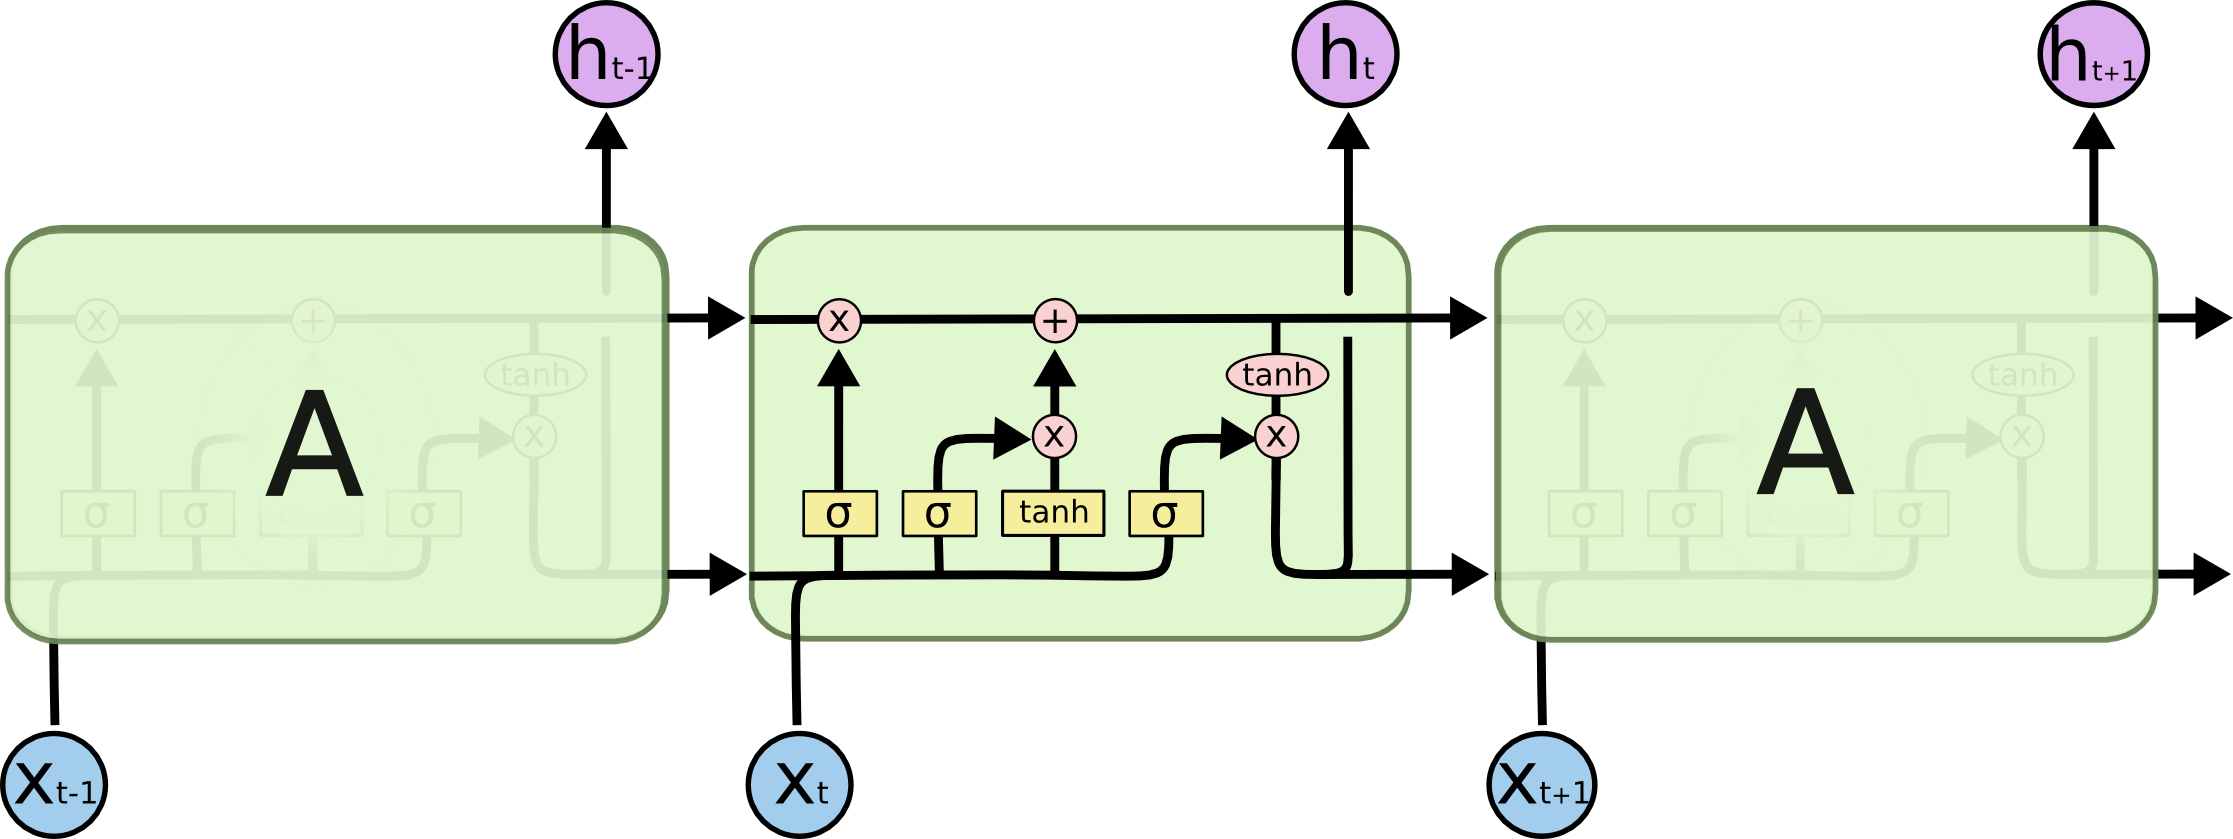
\includegraphics[width=0.5\textwidth]{figures/cv_deep_video_LSTM.png}
		\caption{Visual representation of a LSTM chain.}
		\label{fig:deep_video_LSTM}
	\end{figure}
\end{itemize}
\subsection{3D convolutions}
\begin{itemize}
	\item We can extend standard convolutions to 3D by moving the filter over the time dimension as well (channels are now 4th dimension over which filter is still global)
	\begin{figure}[ht!]
		\centering
		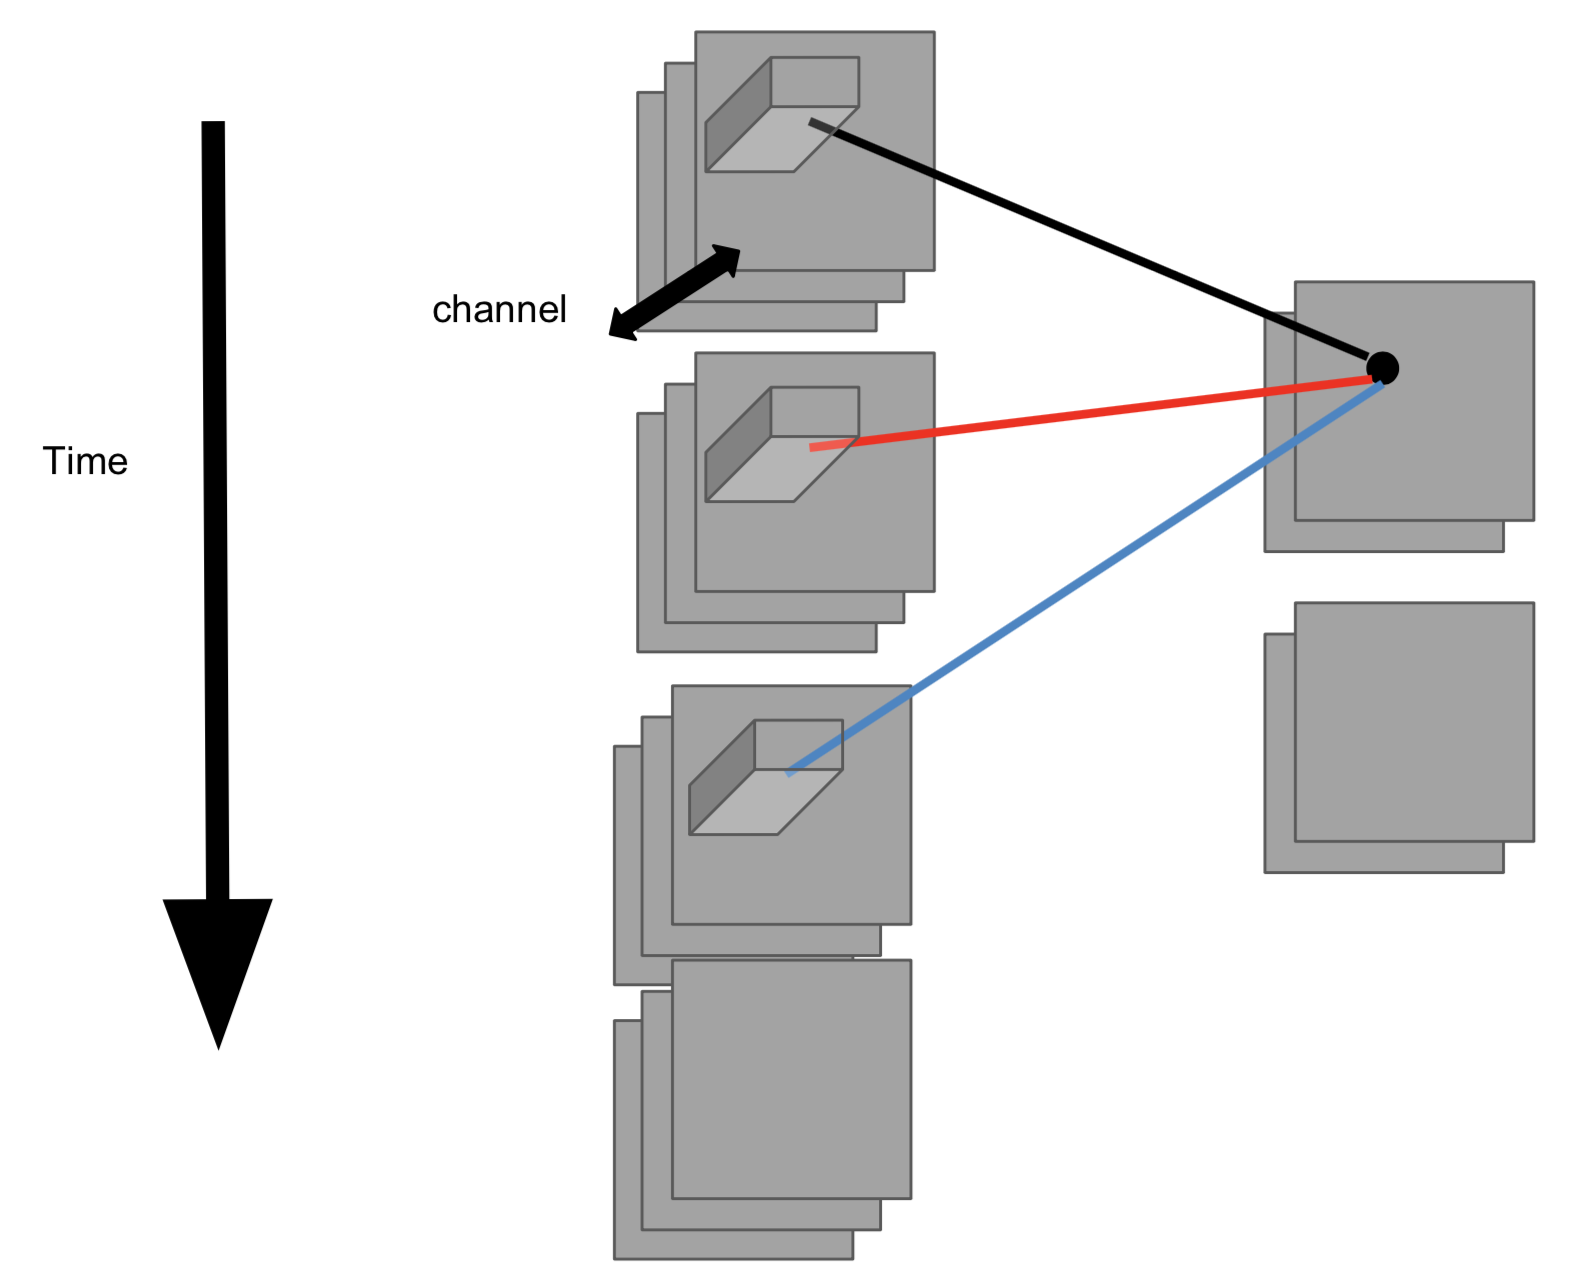
\includegraphics[width=0.3\textwidth]{figures/cv_deep_video_3D_convs.png}
		\caption{A 3D convolution is local over spatial and temporal dimensions, but still global over channels (i.e. RGB).}
		\label{fig:deep_video_3d_convs}
	\end{figure}
	\item Example: extending a 2D kernel by temporal dimension:
	\begin{equation*}
		\begin{split}
			200\times 200\times 3 \textcolor{blue}{\times 16} \xrightarrow{\text{filter }3\times3\textcolor{blue}{\times 3}} 200\times 200\times 256 \textcolor{blue}{\times 16}
			\Rightarrow \underbrace{3\times 3}_{\text{ spatial }}\underbrace{\textcolor{blue}{\times 3}}_{\text{ temporal }}\underbrace{\times 3}_{\text{ input channels }}\underbrace{\times 256}_{\text{ output channels}}\text{ parameters}
		\end{split}
	\end{equation*}
	\item Such convolutions learn combined temporal and spatial information. 
	\item Alternative is to concatenate all input frames over the channel dimension and pass it to a simple 2D network (also called \textit{early fusion}). Note that this approach loses the temporal information very fast
	\item Consecutive 3D convolutions can be seen as hierarchical combination of frames. Low level layers therefore capture low level motions, while high level layers (close to output) are able to reason about a longer set of frames and thus high level motion.
	\item Still, it is hard to learn long term dependencies with 3D convolutions as it does not have any gates and thus no explicit control over the information flow
	\item Note that in general, video-based networks are more likely to suffer from overfitting as the input space has a much higher dimensionality and the network has more parameters
\end{itemize}
\subsection{State-of-the-art}
\subsubsection{Two Stream Network}
\begin{itemize}
	\item Earliest proposed network for action recognition was \textbf{Two stream network}
	\item The architecture consists of two networks. One takes a single frame (\textit{spatial} stream net), and the other processes the concatenated optical flow over the set of frames (\textit{temporal} stream net). Both predictions are in the end combined
	\item The biggest problem here is that the spatial and temporal information is processed independently, and the very late fusion makes it impossible to reason about both
	\item Other disadvantages include a higher computational cost (two networks plus optical flow), only capturing short motion (early fusion of optical flow), noisy optical flow, and higher probability of overfitting due to number of parameters
	\item Approach can be slightly improved by repeatedly applying the network on small snippets of the network, and combining the prediction afterwards
	\begin{figure}[ht!]
		\centering
		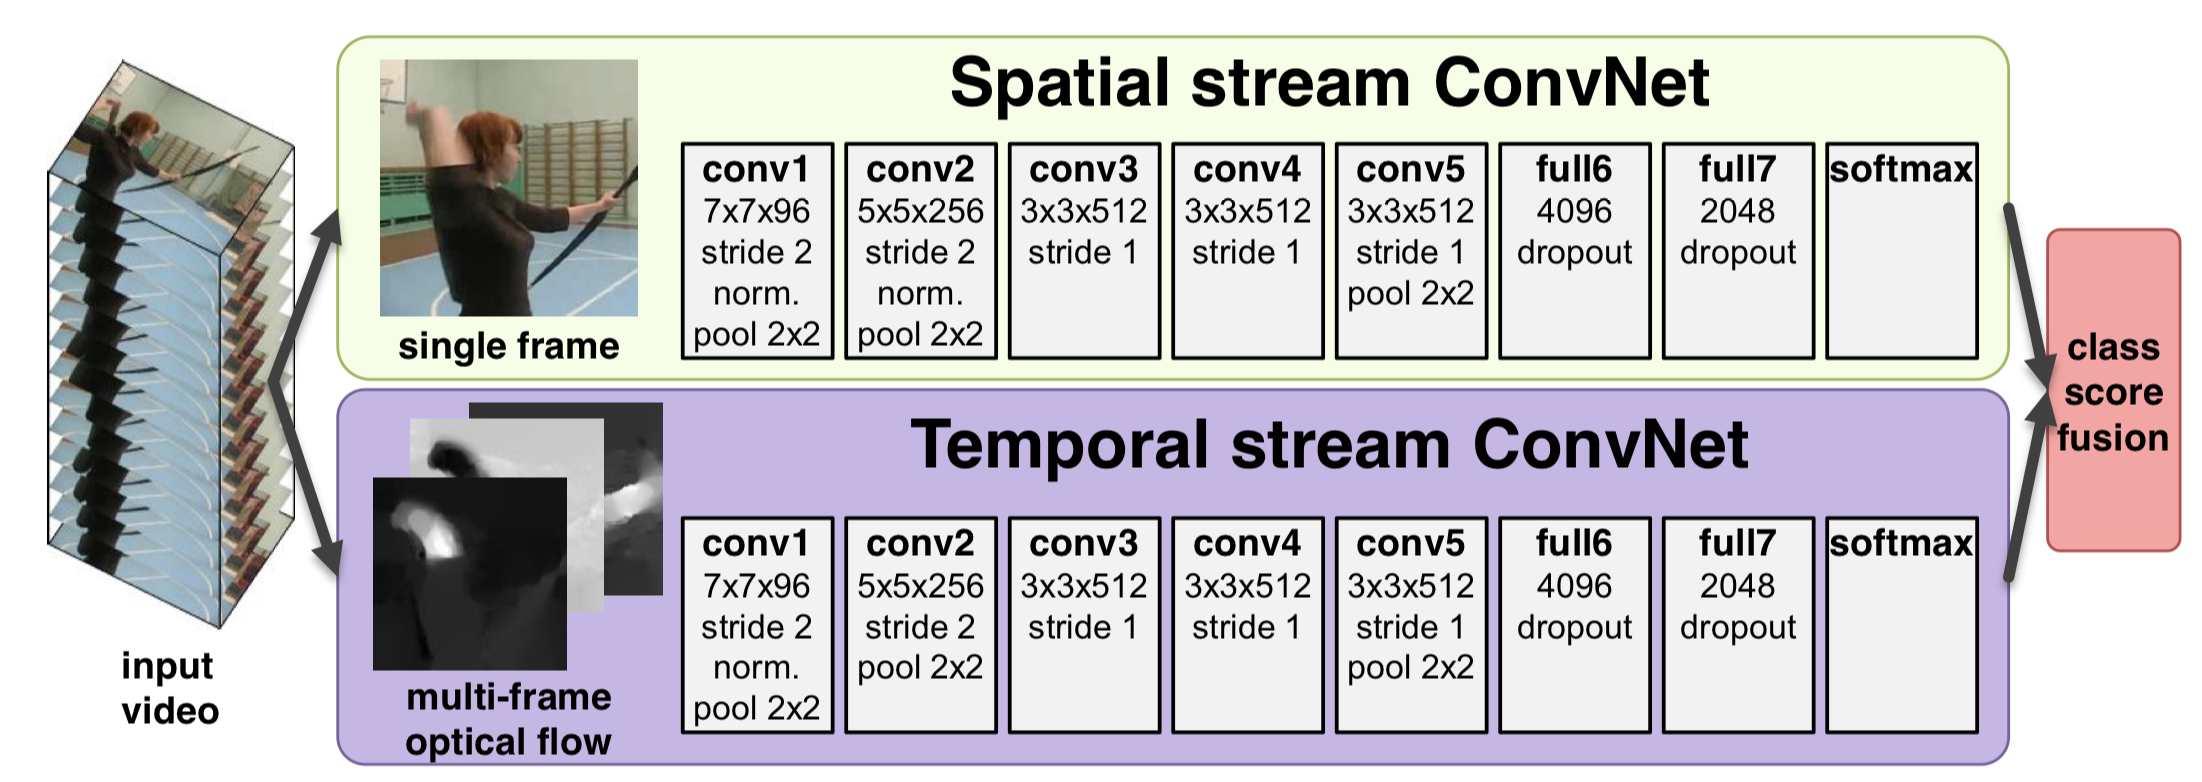
\includegraphics[width=0.5\textwidth]{figures/cv_deep_video_two_stream_network.png}
		\caption{Architecture of the two stream network.}
		\label{fig:deep_video_two_stream_net}
	\end{figure}
\end{itemize}
\subsubsection{I3D}
\begin{itemize}
	\item Inspired by the success of the 2D version (GoogLeNet), current state-of-the-art networks apply 3D inception modules (see Figure~\ref{fig:deep_video_I3D_module})
	\begin{figure}[ht!]
		\centering
		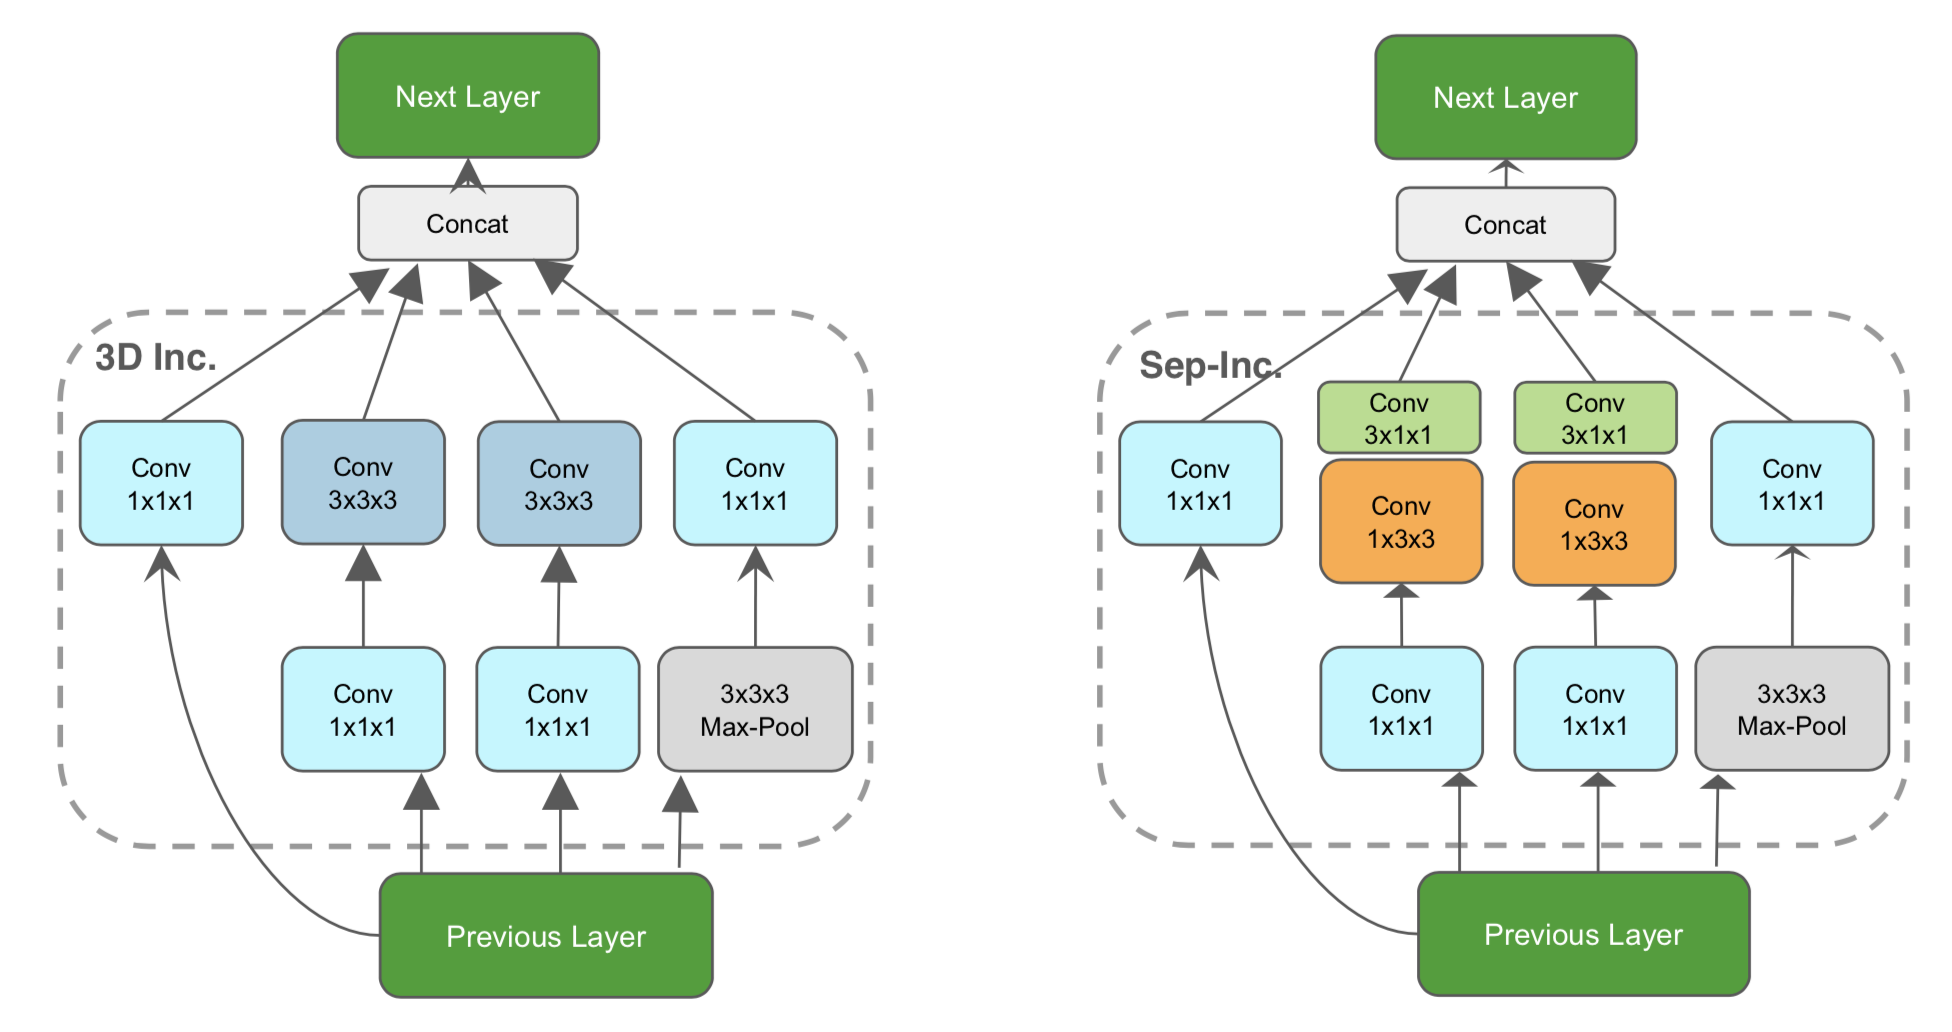
\includegraphics[width=0.35\textwidth]{figures/cv_deep_video_I3D.png}
		\caption{\textit{Left}: Standard Inception module of the I3D network. \textit{Right}: Inception module with 3D temporal separable convolutions.}
		\label{fig:deep_video_I3D_module}
	\end{figure}
	\item It is pretrained on ImageNet where the 2D filters are (after pretraining) inflated to a third dimension by repeating the values $N$ times over the time dimension, and rescaled by dividing by $N$
\end{itemize}
\subsubsection{Efficient 3D convolutions}
\begin{itemize}
	\item The main drawback of I3D and all other 3D convolutional networks are the huge amount of parameters. There are three ways to efficiently reduce the number of parameters
\end{itemize}
\begin{enumerate}
	\item \textbf{Pseudo 3D convolutions}
	\begin{itemize}
		\item The idea behind this operation is that the spatial and the temporal dimension do not correlate in every detail, but the temporal dimension is more important locally for the spatial dimension
		\item Thus, we split 3D convolution into a 2D spatial and a consecutive 1D temporal convolution. The concept is visualized in Figure~\ref{fig:deep_video_pseudo_3D_convs}
		\item The number of operations applied on input size $l_F \times w_F \times h_F \times c_F$ to output $l_G \times w_G \times h_G \times c_G$ is:
		\begin{equation*}
				\underbrace{k \times k \times 1 \times c_F \times c_I \times l_F \times w_G \times h_G}_{\text{Spatial 2D convolution}} + \underbrace{1\times 1\times k \times c_I \times c_G \times l_G \times w_G \times h_G}_{\text{Temporal 1D convolution}}
		\end{equation*}
		\item The speedup by this operation is about $\frac{1}{k}\cdot \frac{c_I}{c_G} \cdot \frac{l_F}{l_G} + \frac{1}{k^2} \cdot \frac{c_I}{c_F}\approx \frac{1}{k}\cdot \frac{c_I}{c_G}$
	\end{itemize}
	\begin{figure}[ht!]
		\centering
		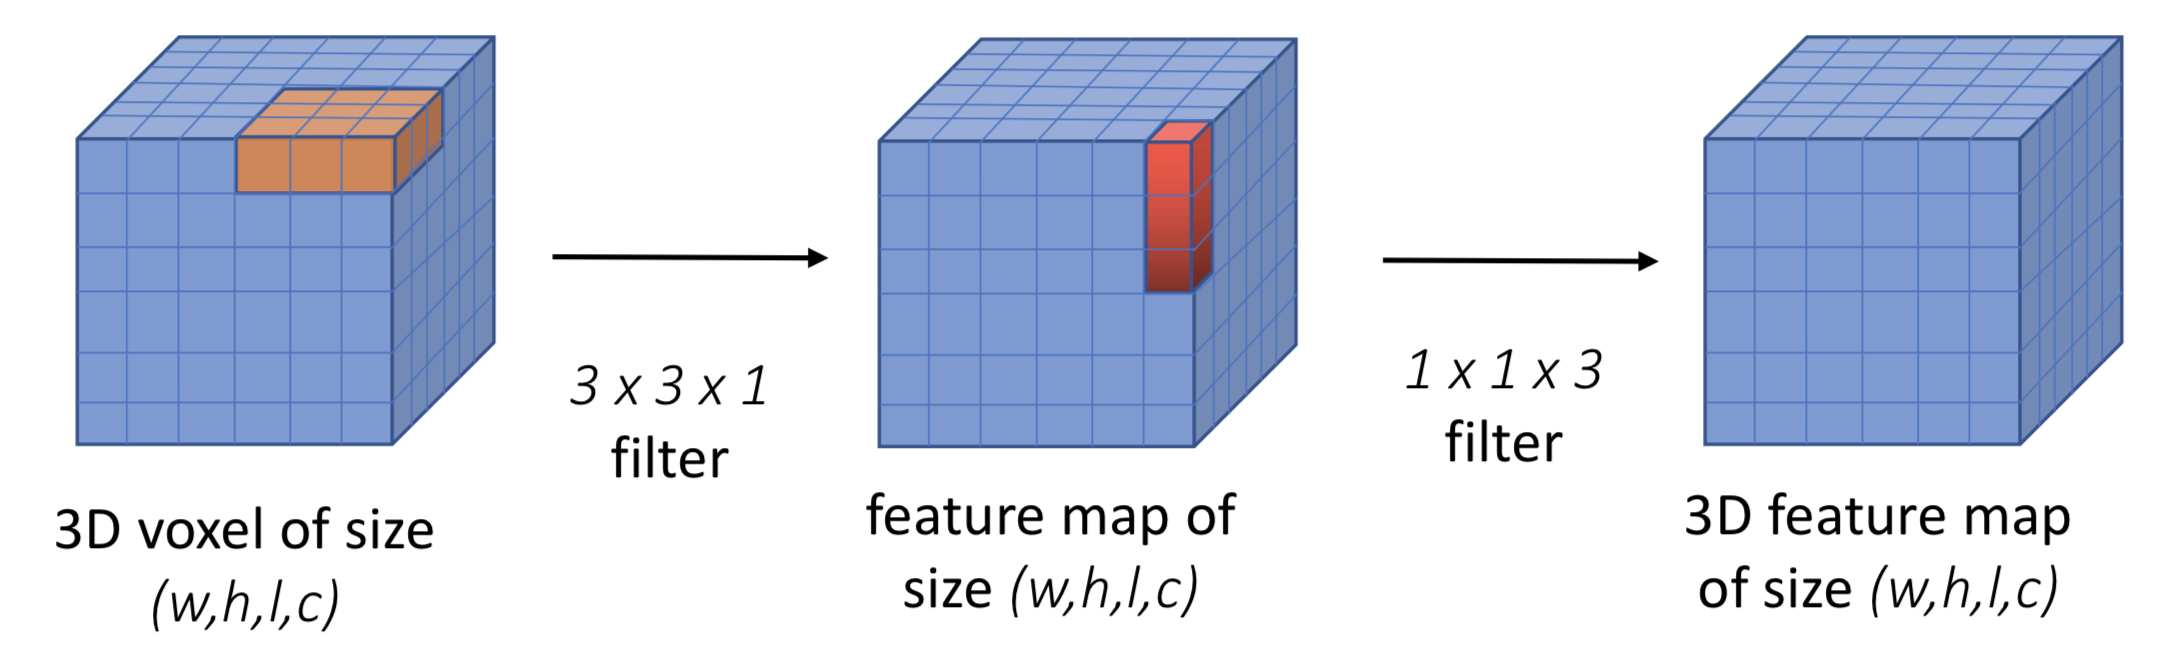
\includegraphics[width=0.55\textwidth]{figures/cv_deep_video_pseudo_3D_conv.png}
		\caption{Pseudo 3D convolutions split the operation into a spatial part (2D) and a temporal (1D) convolution.}
		\label{fig:deep_video_pseudo_3D_convs}
	\end{figure}
	\item \textbf{Depth-wise separable convolutions}
	\begin{itemize}
		\item This operation is inspired by the MobileNet architecture and removes the property of convolutions being depth-wise global
		\item We consider every input channel independently, and apply a different filter on each of them. For example, if we have an RGB input, we would apply three filters, each processing a different input channel
		\item To still allow interaction/combination of multiple channels, we apply a local $1\times 1\times 1$ convolution afterwards. Hence, an output channel depends again on all input channels.
		\item The number of operations applied on input size $l_F \times w_F \times h_F \times c_F$ to output $l_G \times w_G \times h_G \times c_G$ is:
		\begin{equation*}
			\underbrace{k \times k \times k \times 1 \times c_F \times l_G \times w_G \times h_G}_{\text{Depth-wise 3D convolution}} + \underbrace{1\times 1\times 1 \times c_F \times c_G \times l_G \times w_G \times h_G}_{\text{Local }1\times 1\times 1\text{ convolution}}
		\end{equation*}
		\item The speedup by this operation is considerably bigger than for pseudo 3D, namely $\frac{1}{c_G} + \frac{1}{k^{3}} \approx \frac{1}{k^{3}}$
		\begin{figure}[ht!]
			\centering
			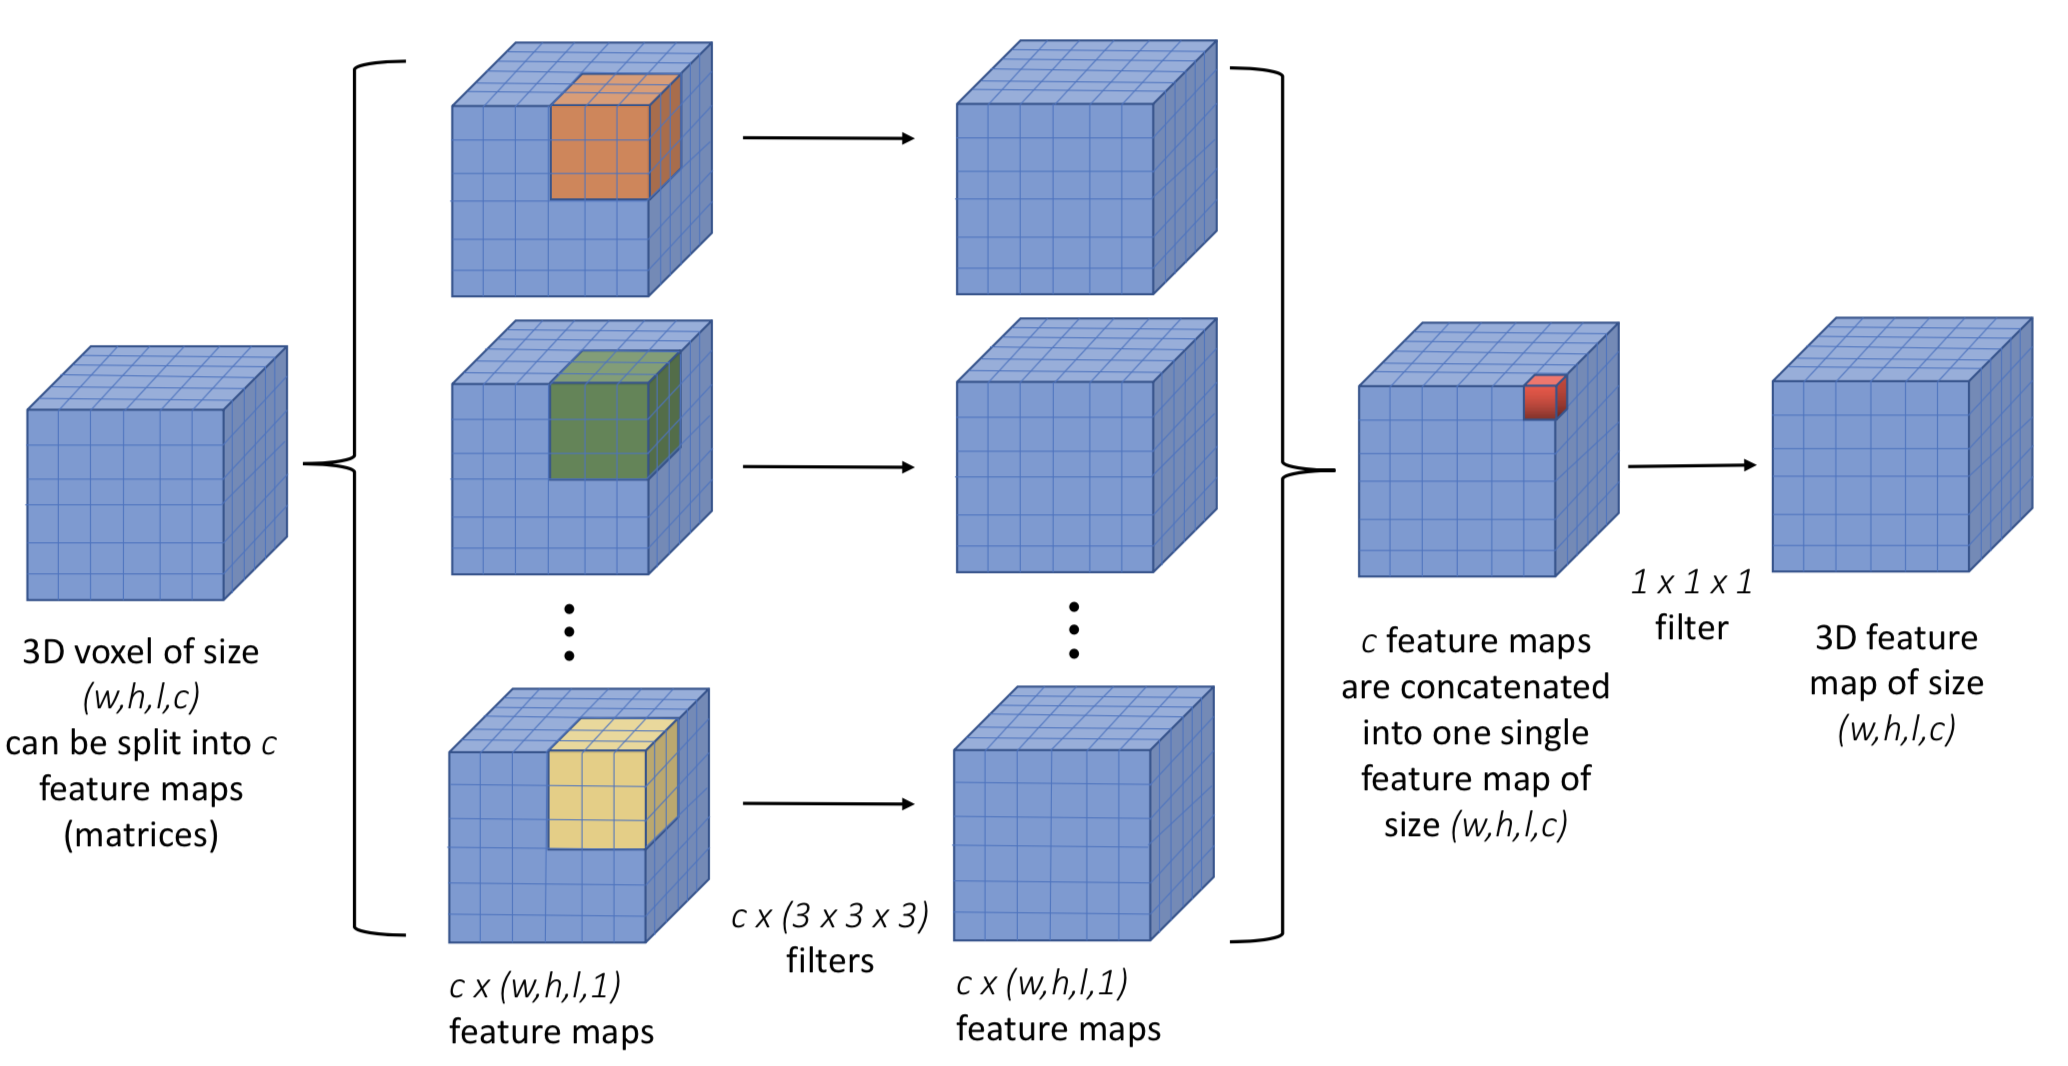
\includegraphics[width=0.6\textwidth]{figures/cv_deep_video_3D_depthwise_conv.png}
			\caption{Depth-wise 3D convolutions apply one filter per input channel, and combine the different channels afterwards. Same architecture is applied in MobileNet for the 2D case.}
			\label{fig:deep_video_depthwise_3D_convs}
		\end{figure}
	\end{itemize}
	\item \textbf{Partial 2D architecture} 
	\begin{itemize}
		\item Depending on the kind of motion we want to detect, it might not be necessary to apply 3D convolutions at every stage of the network. 
		\item For example, if we are only interested in high-level motions, we might want ot use a \textit{Top-heavy I3D} which applies 3D convolutions only on the last layers. 
		\item Similarly, for short motions, we might want to consider a \textit{Bottom-heavy I3D}. 
		\item Figure~\ref{fig:deep_video_I3D_architectures} summarizes the different network architectures.
		\begin{figure}[ht!]
			\centering
			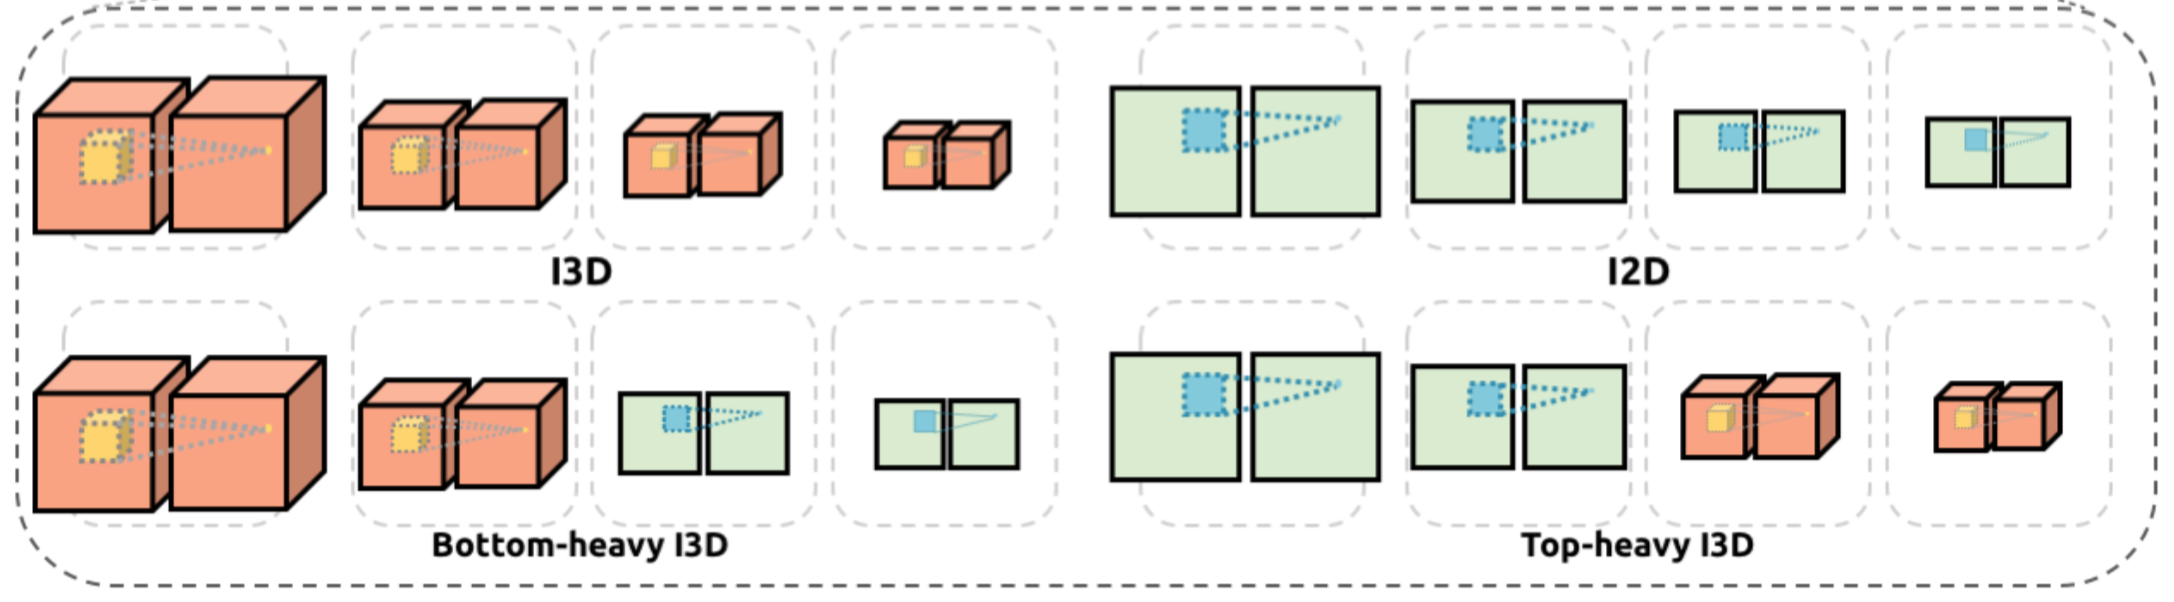
\includegraphics[width=0.6\textwidth]{figures/cv_deep_video_different_I3D_architectures.png}
			\caption{Different I3D network architectures.}
			\label{fig:deep_video_I3D_architectures}
		\end{figure}
	\end{itemize}
\end{enumerate}
\subsection{Self-supervised learning}
\begin{itemize}
	\item Learn to represent a video adequately in the network by using data and tasks where the labels are freely exploited. The great benefit is that we can use a lot of (unlabeled) data
	\item This is mostly done as a pre-training step as the network learns to deal and analyze with videos on a huge dataset. There are various tasks we can perform self-supervised learning on:
	\begin{itemize}
		\item \textbf{Visual tracking}: If we have given a tracking system, we can train a network to predict whether two patches are similar or not. Therefore, we create labels by the tracking system by setting it to 1 if two patches are the same object over time, or otherwise to 0 (we sample a random other patch from the image and compare the scores).
		\item \textbf{Learning by shuffling}: The network is given a set of frames, and its tasks is it to determine whether it is in the correct temporal order or not. The supervision signals are easily generated by labeling the real videos as positive, and shuffle their frame order to create a negative example. The goal is that the network learns to understand poses and motions over frames.
		\item \textbf{Learning by arrow of time}: The task of the network is to predict whether a video is played forwards of backwards (binary classification). This is a very challenging task as it requires the network to understand laws of physics (water only flows downwards, not upwards) by analyzing different motions in the video. One can cluster afterwards what clues the network had extracted which lead to a prediction of forward or backward (called \textit{arrow of time}). This approach gave the best self-supervised pre-training results so far, but is still not able to beat a supervised ImageNet pre-training.   
	\end{itemize}
\end{itemize}